\documentclass{article}
\usepackage[paperwidth=7.4cm,paperheight=5.4cm,margin=1mm]{geometry}
\usepackage[UTF8]{ctex}
\usepackage{amsmath,amssymb,bm}
\usepackage{tikz}
\usetikzlibrary{arrows.meta,calc}
\pagestyle{empty}
\begin{document}
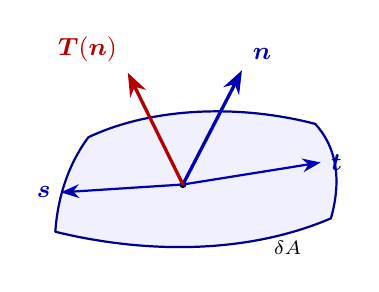
\begin{tikzpicture}[>=Stealth,font=\small,line join=round,line cap=round]
  % ===== 曲面片（斜投影） =====
  \fill[blue!6] (0,0.35)
    .. controls (1.1,0.08) and (2.4,0.05) .. (3.5,0.52)
    .. controls (3.65,1.05) and (3.55,1.45) .. (3.3,1.72)
    .. controls (2.3,1.98) and (1.2,1.92) .. (0.42,1.55)
    .. controls (0.12,1.15) and (0.02,0.68) .. cycle;
  \draw[blue!55!black,thick] (0,0.35)
    .. controls (1.1,0.08) and (2.4,0.05) .. (3.5,0.52)
    .. controls (3.65,1.05) and (3.55,1.45) .. (3.3,1.72)
    .. controls (2.3,1.98) and (1.2,1.92) .. (0.42,1.55)
    .. controls (0.12,1.15) and (0.02,0.68) .. cycle;
  % 面元中心
  \coordinate (P) at (1.62,0.95);
  \fill[black] (P) circle (1.3pt);
  % 法向与两个切向
  \draw[->,very thick,blue!70!black] (P) -- ++(0.75,1.45) node[above right] {$\boldsymbol{n}$};
  \draw[->,thick,blue!70!black] (P) -- ++(1.75,0.28) node[right] {$\boldsymbol{t}$};
  \draw[->,thick,blue!70!black] (P) -- ++(-1.55,-0.10) node[left] {$\boldsymbol{s}$};
  % 应力矢量
  \draw[->,very thick,red!70!black] (P) -- ++(-0.70,1.42) node[above left] {$\boldsymbol{T}(\boldsymbol{n})$};
  % 面元面积
  \node[font=\scriptsize] at (2.95,0.15) {$\delta A$};
\end{tikzpicture}
\end{document}
